\documentclass[border=10pt]{standalone}
\usepackage{tikz}
\begin{document}
	\begin{tikzpicture}[line width=.7pt,x={(1,0)}, y={(0,1)}, z={(-0.5,-0.5)}]
		\coordinate (O)  at (0,0,0);
		\coordinate (x1) at (3,0,0);
		\coordinate (x2) at (0,3,0);
		\coordinate (x3) at (0,0,3);
		\coordinate (x)  at (3,3,3);
		\coordinate (xO) at (3,0,3);
		
		% Draw axes
		\foreach \c in {{4.5,0,0}, {0,4.5,0}, {0,0,4.5}}{
			\draw (O) -- +(\c) ;
		}
		
		% Draw vectors
		\foreach \c/\l/\p in {x1/$x_1$/above, x2/$x_{2}$/left, x3/$x_{3}$/above left}{
			\draw[->,thick] (O) -- +(\c) node[pos=0.7,\p] {\l};
		}
		\draw[->] (O) -- node[pos=0.7,above left] {$\mathbf{x}$} (x);
		
		% Draw helping lines
		\draw[help lines,dashed] (x3) -- ++(x1) -- (x1) (O) -- (xO) -- (x) -- (x2);		
	\end{tikzpicture}
Another figure\\


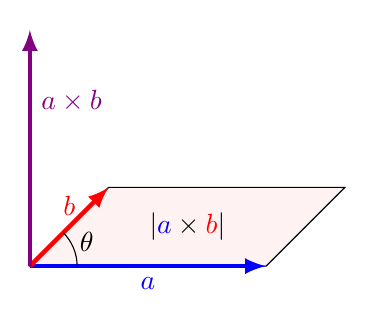
\begin{tikzpicture}
	\draw[-,fill=white!95!red](0,0)--(3,0)--(4,1)--(1,1)--cycle;
	\node at (2,0.5) {$|\textcolor{blue}{a}\times \textcolor{red}{b}|$};
	\draw[ultra thick,-latex,blue](0,0)--(3,0)node[midway,below]{$a$};
	\draw[ultra thick,-latex,red](0,0)--(1,1)node[midway,above]{$b$};
	\draw[ultra thick,-latex,blue!50!red](0,0)--(0,3)node[pos=0.7,right]{$a\times b$};
	\draw (0.6,0) arc [start angle=0,end angle=45,radius=0.6]
	node[pos=0.7,right]{$\theta$};
\end{tikzpicture}


\end{document}